\section{Смешивая стили}
\label{sec:mixing_styles}

Как мы уже заметили, язык программирования имеющий функциональные и
императивные особенности даёт свободу выбора наиболее подходящего стиля для
реализации того или иного алгоритма. Конечно, мы можем использовать оба аспекта
Objective CAML совместно в одной и той же функции. Именно этим мы сейчас и
займёмся.

\subsection{Замыкания и побочные эффекты}
\label{subsec:closures_and_side_effects}

Обычно функция с побочным эффектом рассматривается как процедура и она
возвращает значение () типа \texttt{unit}. Однако, иногда бывает полезно
произвести побочный эффект внутри функции и вернуть определённое значение. Мы
уже использовали подобный коктейль стилей в функции \texttt{permute\_pivot} в
быстрой сортировке.

В следующем примере реализуем генератор символов, который создаёт новый символ
при каждом вызове функции. Мы используем счётчик, значение которого
увеличивается с каждым вызовом.

\begin{lstlisting}[language=OCaml]
# let c = ref 0;;
val c : int ref = {contents = 0}
# let reset_symb = function () -> c:=0 ;;
val reset_symb : unit -> unit = <fun>
# let new_symb = function s ->  c:=!c+1 ; s^(string_of_int !c) ;;
val new_symb : string -> string = <fun>
# new_symb "VAR" ;;
- : string = "VAR1"
# new_symb "VAR" ;;
- : string = "VAR2"
# reset_symb () ;;
- : unit = ()
# new_symb "WAR" ;;
- : string = "WAR1"
# new_symb "WAR" ;;
- : string = "WAR2"
\end{lstlisting}

А теперь спрячем ссылку на c от всей программы следующим образом:

\begin{lstlisting}[language=OCaml]
# let (reset_s , new_s) =
   let c = ref 0
   in let f1 () = c := 0
      and f2 s  = c := !c+1 ; s^(string_of_int !c)
   in (f1,f2) ;;
val reset_s : unit -> unit = <fun>
val new_s : string -> string = <fun>
\end{lstlisting}

Таким образом мы объявили пару функций, разделяющие локальную (для декларации)
переменную \texttt{c}. Использование обеих функций производит тот же результат
что и раньше.

Этот пример иллюстрирует способ представления замыкания. Замыкание можно
рассматривать как пару, состоящую из кода (то есть часть \texttt{function}) и
локальное окружение, содержащее значения свободных переменных замыкания с другой
стороны. На диаграмме \ref{fig:memory_representation_of_closures} мы можем
увидеть представление в памяти замыканий \texttt{reset\_s} и \texttt{new\_s}.

\begin{figure}[h]
	\center{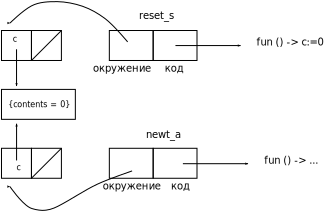
\includegraphics[width=\textwidth]
{img/memory_representation_of_closures}}
	\caption{\label{fig:memory_representation_of_closures}Представление в памяти 
замыканий}
\end{figure}

Оба эти замыкания разделяют одно и тоже окружение (значение \texttt{c}). Когда
одно из них меняет ссылку \texttt{c}, то оно меняет содержимое памяти
разделяемое с другим окружением.

\subsection{Физическое изменение и исключения}
\label{subsec:physical_modifications_and_exceptions}

 Исключения позволяет отслеживать ситуацию, при которой дальнейшее продолжение
программы невозможно. В подобном случае сборщик исключений позволит продолжить
вычисление, зная что произошла ошибка. В момент возбуждения исключения может
возникнуть проблема побочного эффекта с состоянием модифицируемых данных. Это
состояние не может быть гарантированно если произошли физические изменения в
ответвлении неудавшегося вычисления.

Определим функцию увеличения (++), с аналогичным результатом что и в C:

\begin{lstlisting}[language=OCaml]
# let (++) x = x:=!x+1; x;;
val ( ++ ) : int ref -> int ref = <fun>
\end{lstlisting}

Следующий пример, иллюстрирует небольшой расчёт в котором деление на ноль
совпадает с побочным эффектом:

\begin{lstlisting}[language=OCaml]
# let x = ref 2;;
val x : int ref = {contents = 2}
# !((++) x) * (1/0) ;;
Exception: Division_by_zero.
# x;;
- : int ref = {contents = 2}
# (1/0) * !((++) x) ;;
Exception: Division_by_zero.
# x;;
- : int ref = {contents = 3}
\end{lstlisting}

Переменная \texttt{x} не изменяется во время вычисления выражения (*1*), тогда
как она изменяется во время (*2*). Если заранее не сохранить начальные значения,
конструкция \texttt{try .. with ..} не должна (в части \texttt{with ..})
зависеть от изменяемых переменных, которые участвуют в вычислении возбудившем
исключение.

\subsection{Изменяемые функциональные структуры данных}
\label{subsec:modifiable_functional_data_structures}

В функциональном программирование программа, как функциональное выражение,
является в то же время данными --- чтобы уяснить этот момент напишем список
ассоциированных значений в виде функционального выражения. Этот список
ассоциаций \texttt{('a * 'b) list} можно рассматривать как частичную функцию из
\texttt{'a} (множество ключей) в \texttt{'b} (множество соответствующих
значений). Другими словами, функция \texttt{'a -> 'b}.

Пустой список это неопределённая функция, которую мы будем моделировать
возбуждением исключения:

\begin{lstlisting}[language=OCaml]
# let nil_assoc = function x -> raise Not_found ;;
val nil_assoc : 'a -> 'b = <fun>
\end{lstlisting}

Теперь напишем функцию \texttt{add\_assoc} добавляющую элемент в список или
другими словами расширим функцию новыми значениями.

\begin{lstlisting}[language=OCaml]
# let add_assoc (k,v) l = function x -> if x = k then v else l x ;;
val add_assoc : 'a * 'b -> ('a -> 'b) -> 'a -> 'b = <fun>
# let l = add_assoc ('1', 1) (add_assoc ('2', 2) nil_assoc) ;;
val l : char -> int = <fun>
# l '2' ;;
- : int = 2
# l 'x' ;;
Exception: Not_found.
\end{lstlisting}

Перепишем функцию \texttt{mem\_assoc}:

\begin{lstlisting}[language=OCaml]
# let mem_assoc k l = try  (l k) ; true  with  Not_found -> false ;;
val mem_assoc : 'a -> ('a -> 'b) -> bool = <fun>
# mem_assoc '2' l ;;
- : bool = true
# mem_assoc 'x' l ;;
- : bool = false
\end{lstlisting}

Однако, написание функции удаляющей элементы из списка, не совсем простое дело.
У нас больше нет доступа к значениям входящим в замыкание. Для этого мы спрячем
старое значение возбудив исключения \texttt{Not\_found}.

\begin{lstlisting}[language=OCaml]
# let rem_assoc k l = function x -> if x=k then raise Not_found else l x ;;
val rem_assoc : 'a -> ('a -> 'b) -> 'a -> 'b = <fun>
# let l = rem_assoc '2' l ;;
val l : char -> int = <fun>
# l '2' ;;
Exception: Not_found.
\end{lstlisting}

Естественно, можно воспользоваться ссылками и побочным эффектом для
использования таких значений, однако существует несколько предостережений.

\begin{lstlisting}[language=OCaml]
# let add_assoc_again (k,v) l =  l := (function x -> if x=k then v else !l x) ;;
val add_assoc_again : 'a * 'b -> ('a -> 'b) ref -> unit = <fun>
\end{lstlisting}

Мы получили функцию \texttt{l} которая указывает сама на саму себя и значит
будет зацикливаться. Этот досадный побочных эффект есть результат того что
разыменование \texttt{!l} находится внутри замыкания \texttt{function x ->}.
Значение \texttt{!l} вычислено при выполнении, а не компиляции. В этот момент,
\texttt{l} указывает на значение изменённое \texttt{add\_assoc}. Необходимо
исправить наше определение используя замыкание полученное определением
\texttt{add\_assoc}:

\begin{lstlisting}[language=OCaml]
# let add_assoc_again (k, v) l =  l := add_assoc (k, v) !l ;;
val add_assoc_again : 'a * 'b -> ('a -> 'b) ref -> unit = <fun>
# let l = ref nil_assoc ;;
val l : ('_a -> '_b) ref = {contents = <fun>}
# add_assoc_again ('1',1) l ;;
- : unit = ()
# add_assoc_again ('2',2) l ;;
- : unit = ()
# !l '1' ;;
- : int = 1
# !l 'x' ;;
Exception: Not_found.
\end{lstlisting}

\subsection{Ленивые изменяемые структуры}
\label{subsec:lazy_modifiable_data_structures}

Смесь императивных особенностей с функциональным языком образует хорошие
средства реализации языков программирования. В данном параграфе мы
проиллюстрируем эту особенность в реализации структур данных с отсроченным
вычислением. Такая структура данных не вычисляется полностью, вычисление
продвигается в зависимости от использования структуры.

Отложенное вычисление, часто используемое в чистых функциональных языках, можно
моделировать использованием функциональных значений (возможно, изменяемых).
Выгода от использования данных с отложенным выполнением двойная; во первых
вычисляется лишь то что необходимо для расчёта, во вторых использование
потенциально бесконечных данных.

Определим тип \texttt{vm} элементы которого либо уже вычисленное значение
(конструктор \texttt{Imm}) либо значение которое будет вычислено (конструктор
\texttt{Deferred}).

\begin{lstlisting}[language=OCaml]
# type 'a v =
     Imm of 'a
   | Deferred of (unit -> 'a);;
type 'a v = Imm of 'a | Deferred of (unit -> 'a)
# type 'a vm = {mutable c : 'a v };;
type 'a vm = { mutable c : 'a v; }
\end{lstlisting}

Откладывание вычислений может быть получено инкапсуляцией в замыкание. Функция
вычисляющая такое значение должна или вернуть значение если оно уже вычислено
или, в противном случае, вычислить и сохранить результат.

\begin{lstlisting}[language=OCaml]
# let eval e = match e.c with
   Imm a -> a
 | Deferred f -> let u = f () in e.c <- Imm u ; u ;;
val eval : 'a vm -> 'a = <fun>
\end{lstlisting}

Операции задержки и активации вычисления также называют замораживанием и
размораживанием значения.

Напишем условный контроль в виде функции:

\begin{lstlisting}[language=OCaml]
# let if_deferred c e1 e2 =
   if eval c then eval e1 else eval e2;;
val if_deferred : bool vm -> 'a vm -> 'a vm -> 'a = <fun>
\end{lstlisting}

А теперь воспользуемся этим в рекурсивной функции подсчёта факториала.

\begin{lstlisting}[language=OCaml]
# let rec facr n =
   if_deferred
          {c=Deferred(fun () -> n = 0)}
          {c=Deferred(fun () ->  1)}
          {c=Deferred(fun () -> n*(facr(n-1)))};;
val facr : int -> int = <fun>
# facr 5;;
- : int = 120
\end{lstlisting}

Заметим, что классический \texttt{if} не может быть записан в виде функции.
Действительно, определим функцию \texttt{if\_function} следующим образом:

\begin{lstlisting}[language=OCaml]
# let if_function c e1 e2 = if c then e1 else e2;;
val if_function : bool -> 'a -> 'a -> 'a = <fun>
\end{lstlisting}

Дело в том что все три аргумента вычисляются, это приводит к зацикливанию, так
как рекурсивный вызов \texttt{fact(n - 1)} всегда вычисляется, даже в случае
когда \texttt{n = 0}.

\begin{lstlisting}[language=OCaml]
# let rec fact n = if_function (n=0) 1 (n*fact(n-1)) ;;
val fact : int -> int = <fun>
# fact 5 ;;
Stack overflow during evaluation (looping recursion?).
\end{lstlisting}

\subsubsection{Модуль Lazy}

Трудности во внедрении замороженных значений происходят от конструкции выражений
с отложенным вычислением в контексте немедленного вычисления Objective CAML. Мы
это увидели при попытке переопределить условное выражение. Нельзя написать
функцию замораживающую значение при конструкции объекта типа \texttt{vm}.

\begin{lstlisting}[language=OCaml]
# let freeze e = { c = Deferred (fun () -> e) };;
val freeze : 'a -> 'a vm = <fun>
\end{lstlisting}

Эта функция следует стратегии вычисления Objective CAML, то есть выражение
\texttt{e} вычисляется перед тем как создать замыкание \texttt{fun () ->e}.
Проиллюстрируем это в следующем примере:

\begin{lstlisting}[language=OCaml]
# freeze (print_string "trace"; print_newline(); 4*5);;
trace
- : int vm = {c = Deferred <fun>}
\end{lstlisting}

По этой причине была введена следующая синтаксическая форма:

Синтаксис

\begin{lstlisting}[language=OCaml]
lazy expr
\end{lstlisting}

\subsubsection{Предупреждение}

Это особенность является расширением языка и может измениться в следующих
версиях.

Когда к выражению применяется ключевое слово \texttt{lazy} то создаётся значение
особого типа, который определён в модуле \texttt{Lazy}:

\begin{lstlisting}[language=OCaml]
# let x = lazy (print_string "Hello"; 3*4) ;;
val x : int lazy_t = <lazy>
\end{lstlisting}

Выражение (\texttt{print\_string "Hello"}) не вычислено, так как не было
никакого вывода на экран. При помощи функции \texttt{Lazy.force} мы можем
вынудить вычисление выражения.

\begin{lstlisting}[language=OCaml]
# Lazy.force x ;;
Hello- : int = 12
\end{lstlisting}

Тут мы замечаем, что значение x изменилось:

\begin{lstlisting}[language=OCaml]
# x ;;
- : int lazy_t = <lazy>
\end{lstlisting}

Теперь это значение замороженного выражения, в данном случае 12.

Новый вызов функции \texttt{force} просто возвращает вычисленное значение:

\begin{lstlisting}[language=OCaml]
# Lazy.force x ;;
- : int = 12
\end{lstlisting}

Строка \texttt{"Hello"} больше не выводится на экран.

\subsubsection{\enq{Бесконечные} структуры данных}

Другой интерес использования отложенного вычисления состоит в возможности
построения потенциально бесконечных структур данных, как на пример множество
натуральных чисел. Вместо того чтобы конструировать каждое число, мы определим
лишь первый элемент и способ получения следующего.

Определим настраиваемую (\texttt{generic}) структуру \texttt{'a enum} с помощью
которой мы будем определять элементы множества.

\label{subsubsec:infinite_data_structures}

\begin{lstlisting}[language=OCaml]
# type 'a enum = { mutable i : 'a; f :'a -> 'a } ;;
type 'a enum = { mutable i : 'a; f : 'a -> 'a; }
# let next e = let x = e.i in e.i <- (e.f e.i) ; x ;;
val next : 'a enum -> 'a = <fun>
\end{lstlisting}

Для того, чтобы получить множество натуральных достаточно конкретизировать
(\texttt{instanciating}) поля этой структуры.

\begin{lstlisting}[language=OCaml]
# let nat = { i=0; f=fun x -> x + 1 };;
val nat : int enum = {i = 0; f = <fun>}
# next nat;;
- : int = 0
# next nat;;
- : int = 1
# next nat;;
- : int = 2
\end{lstlisting}

Другой пример --- ряд чисел Фибоначчи, который определён как:

$$
\begin{cases}
	u_0 = 1 \\
	u_1 = 1 \\
	u_{n + 2} = u_{n} + u_{n+1};
\end{cases}
$$

Функция, вычисляющая текущее значение, должна использовать значения $u_n - 1$ и
$u_n - 2$. Для этого воспользуемся состоянием \texttt{c} в следующем замыкании.

\begin{lstlisting}[language=OCaml]
# let fib = let fx = let c = ref 0 in fun v -> let r = !c + v in c:=v ; r
           in { i=1 ; f=fx } ;;
val fib : int enum = {i = 1; f = <fun>}
# for i=0 to 10 do  print_int (next fib); print_string "  " done ;;
1  1  2  3  5  8  13  21  34  55  89  - : unit = ()
\end{lstlisting}